\documentclass{article}

%%%%%%%%%%%%%%% LIBRERIAS %%%%%%%%%%%%%%%%%%%%%
\usepackage[thinc]{esdiff}
\usepackage{amsmath}
\usepackage{caption}
\usepackage{physics}
\usepackage{titlesec}
\usepackage{titletoc}
\usepackage{graphicx}
\usepackage[spanish,es-tabla]{babel} % 'es-tabla' cambia Cuadro→Tabla
\usepackage{hyperref}                % cargar después de babel
\usepackage{float}
\usepackage{circuitikz}
\usepackage[left=3cm,right=3cm]{geometry} %para margenes
\usepackage{subfiles} 
\usepackage{subcaption}
\usepackage{booktabs} % Para tablas con tematica de paper cientifico
\usepackage{siunitx}  % Para alinear números en las tablas d:
\usepackage{grffile}
\usepackage{comment} %permite hacer comentrios 


%%%%para graficar csv de una%%%%
\usepackage{pgfplots}
\pgfplotsset{compat=1.18}
\usepackage{pgfplotstable}
\usepgfplotslibrary{groupplots}

%%%%%%%%%%%%%%

%%%%%%%%%%%%%%%%%%% VARIABLES %%%%%%%%%%%%%%%%%%%%
\newcommand{\Facultad}{Instituto Tecnológico \\de\\ Buenos Aires} %constantes
\newcommand{\TPn}{Trabajo Práctico N° 2}								%%%%%NOMBRE DEL TP%%%%%%%%
\newcommand{\TPtema}{Osciloscopios - Analizador de Impedancias}
\renewcommand{\thesection}{\arabic{section}}          % 2
\renewcommand{\thesubsection}{\quad \alph{subsection}}   % a
\renewcommand{\thesubsubsection}{\quad \thesubsection.~\roman{subsubsection}} % a. i
\graphicspath{{imagenes/}} %para que acceda a las fotos en la carpeta directamente


%%%%%%%%%%%%%%%%%% FORMATO TÍTULO Y NUMERACIÓN %%%%%%%%%%%%%%%%%%%
% Numeración de secciones
\renewcommand{\thesection}{\arabic{section}.}          
\renewcommand{\thesubsection}{\thesection\arabic{subsection}}       
\renewcommand{\thesubsubsection}{$\alph{subsubsection})$}

% Numerar hasta subsubsecciones
\setcounter{secnumdepth}{3}

% Formato de títulos
\titleformat{\section}{\LARGE\bfseries}{\thesection}{1em}{}
\titleformat{\subsection}{\large\bfseries}{\thesubsection}{0.5em}{}
\titleformat{\subsubsection}{\large\bfseries}{\thesubsubsection}{0.5em}{}
%%
%
% \pgfplotstableread[col sep = comma]{data.csv}\data    LEE EL ARCHIVO.CSV Y LO GUARDA EN LA VARIABLE "\data"
%
%
%
%
%


%%%%%%%%%%%%%%%%%%% ARCHIVO %%%%%%%%%%%%%%%%%%%%%%%%
\begin{document}

%%%CARATULA%%%
\begin{titlepage} %creo portada

        \begin{flushleft}
            \centering
            
\includegraphics[width=0.3\textwidth]{Logo_ITBA.png}
        \end{flushleft}

        \centering
            
        {\scshape\LARGE \Facultad \par} %\par sirve para indicar un final de parrafo
        \vspace{1cm}                    %esto hace un espacio entre lineas de 1cm


        {\huge\bfseries \TPn \par}
        \vspace{1.5cm}
        {\Large Laboratorio de Electrónica\\ 25.13 \par}
        \vspace{0.5cm}
        {\Large \TPtema \par}
        \vfill                      %sirve para rellenar el espacio y quede simétrico.
        {\Large \bfseries Grupo N° 2 \par}
        \vspace{1cm}
        {\large Juan Bautista Correa Uranga \hfill Legajo: 65016 \par} 
        {\large Juan Ignacio Caorsi \hfill Legajo: 65532  \par}
        {\large Rita Moschini \hfill Legajo: 67026 \par} 
        {\large Lucas Solar Grillo \hfill Legajo: 63322\par}
        \vfill
        {\large \today\par}
        \vfill

\end{titlepage}

\tableofcontents 
\newpage

%%%%%%%%%%%%%%%%%%% CUERPO DEL INFORME %%%%%%%%%%%%%%%%%%%%%%%%

\section*{Objetivos} 
El objetivo de este trabajo práctico es profundizar el entendimiento de circuitos de segundo orden, estudiando su naturaleza de filtro a partir de modificaciones hechas sobre un RLC convencional.
Además, se analiza el desempeño del inductor y el capacitor en general.
\section{Instrumentos y equipo}

\begin{minipage}[t]{0.48\textwidth}
    \begin{itemize}
        \setlength{\itemsep}{2pt} % Ajusta el espacio vertical si querés compactarlo más
        \item Protoboard de 830 puntos
        \item Capacitor de 8,2 nF
        \item Resistencia de 68 $\Omega$
        \item Inductor de L 38,76uH
        \item Osciloscopio digital Keysight DSOX1202G
    \end{itemize}
\end{minipage}% <-- Este porcentaje es clave para evitar que la siguiente minipage salte de línea
\hfill % Rellena el espacio horizontal entre las dos columnas
\begin{minipage}[t]{0.48\textwidth}
    \begin{itemize}
        \setlength{\itemsep}{2pt}
        \item Generador de señales Picotest G510
        \item Generador de señales Keysight EDU33212A
        \item Medidor RLC UNI-T UT812
        \item Digilent 
    \end{itemize}
\end{minipage}
    
\section{Inductor}
    
    En la materia TME se calculó un transformador que cumplía ciertos criterios. Para este TP, solo se bobinó el primario. Para ello, este contó con los siguientes parametros:
    \begin{itemize}
\item Nucleo TDK RM10, material N30
\item N1=10
\item Se bobinaron 3 cables en paralelo de 0,45mm de diametro.
\item $L_{gap}$ = 0,3 mm
\end{itemize}

	El valor del inductor medido 38,76 $\mu H$
\section{Cálculo de RLC serie}
A partir de los valores de inductor y capacitor, se calculó el valor 
de la resistencia para que el circuito RLC serie tenga un coeficiente 
de amortiguamiento $\xi=0.5$. Para esto, se utilizó la fórmula
 $\xi = \frac{R}{2} \sqrt{\frac{C}{L}}$. De esta forma, se obtuvo un valor comercial cercano
 de $R = 68 $ $\Omega$. Además, notar que la frecuencia de resonancia del circuito es $f_0 = \frac{1}{2\pi \sqrt{LC}} = 282,3$ kHz.


 %%%%%%%% EJERCICIO 3 %%%%%%%%%%

Utilizando el osciloscopio y el analizador de impedancias de Digilent, se realizó un barrido de frecuencias tanto del inductor como del capacitor, obteniendo los datos visibles en las tablas \ref{tabla:inductancias} y \ref{tabla:inductancias}.

\begin{figure}[H]
    \begin{centering}
        %\begin{tabular}{lcccc}
        %\toprule
        %f (Hz) & L (H) & Q & $ R_s (\Omega)$ & $ \theta (^\circ) $ \\
        %\midrule
        %10, 50, 200, 1k, 10k, 20k, 50k, 100k, 200k, 400k, 600k, 1M
        %\bottomrule
        %\end{tabular}
        \label{tabla:inductancias}
        \caption{Tabla de las inductancias del bobinado y sus valores parásitos a distintas frecuencias.}
    \end{centering}
\end{figure}


\begin{figure}[H]
    \begin{centering}
        %\begin{tabular}{lcccc}
        %\toprule
        %f (Hz) & C (H) & D $ (\cdot 10^{-3}) $ & $ R_p k(\Omega)$ & $ \theta (^\circ) $ \\
        %\midrule
        %\bottomrule
        %\end{tabular}
        \label{tabla:capacitancias}
        \caption{Tabla de las capacitancias del capacitor y sus valores parásitos a distintas frecuencias.}
    \end{centering}
\end{figure}

Con el fin de comparar la impedancia medida y la teórica de cada componente, también se midió y graficó el módulo y la fase de la misma

\begin{figure}[H]
    \begin{centering}
        \begin{tabular}{lccc}
        \toprule
        f (Hz) & $|Z_L|$ & $fase(Z_L)$ \\
        \midrule
        10   & 0.0146 & 10.844 \\
        50   & 0.0188 & 43.809 \\
        200  & 0.054 & 75.409 \\
        1k   & 0.272  & 86.749 \\
        10k  & 2.199   & 89.322 \\
        20k  & 5.615   & 89.49 \\
        50k  & 11.329   & 89.615 \\
        100k & 22.893   & 89.637 \\
        200k & 46.299   & 89.474 \\
        400k & 93.929   & 88.926 \\
        600k & 150.856   & 88.49 \\
        1M   & 244.121   & 87.52 \\
        \bottomrule
        \end{tabular}
        \label{tabla:impedanciaInductiva}
        \caption{Tabla de las inductancias del bobinado y sus valores parásitos a distintas frecuencias.}
    \end{centering}
\end{figure}

Existen múltiples modelos teóricos para un inductor, pero el más simple de todos consiste en un inductor con una resistencia en serie, representando la resistividad del cable de cobre que lo conforma. Acorde a lo estudiado en la materia Tecnología de los Materiales Electrónicos, se obtuvo el valor de la misma mediante la ecuación
\begin{equation*}
    R = \rho \frac{l}{A}
\end{equation*}
donde  l es la longitud del cable que conforma al inductor, A es su área transversal, y $\rho$ su resistividad a determinada temperatura. De esta manera obtuvo el modelo de la figura \ref{modeloTeoricoL}

\begin{figure}[H]
    \begin{tikzpicture}[transform shape]
        % Paths, nodes and wires:
        \draw (1.5, 4) to[sinusoidal voltage source] (1.5, 2);
        \draw (2.5, 4) to[american resistor] (5.25, 4);
        \draw (6.25, 4) to[american inductor] (6.25, 2);
        \draw (6.25, 2) -- (1.5, 2);
        \node[ground] at (1.5, 2){};
        \node[circ] at (2.5, 4){};
        \node[shape=rectangle, minimum width=0.965cm, minimum height=0.215cm] at (2.5, 4.375){} node[anchor=north west, align=left, text width=0.577cm, inner sep=6pt] at (2, 4.5){out};
        \draw (1.5, 4) -- (2.5, 4);
        \draw (5.25, 4) -- (6.25, 4);
        \node[shape=rectangle, minimum width=1.465cm, minimum height=0.465cm] at (4.5, 4.75){};
        \node[shape=rectangle, draw, line width=1pt, minimum width=-0.035cm, minimum height=-0.035cm] at (0, -0){};
        \node[shape=rectangle, minimum width=1.465cm, minimum height=0.465cm] at (4.25, 4.5){} node[anchor=north west, align=left, text width=1.077cm, inner sep=6pt] at (3.5, 4.75){19.1e-3};
        \node[shape=rectangle, minimum width=1.465cm, minimum height=0.465cm] at (7.25, 3){} node[anchor=north west, align=left, text width=1.077cm, inner sep=6pt] at (6.5, 3.25){39.26e-6};
    \end{tikzpicture}
    \caption{Modelo teórico del inductor.}
    \label{modeloTeoricoL}
\end{figure}

Utilizando dicho modelo, se obtuvo una curva teórica semejante a la medida, como se puede observar en las figuras \ref{fig:moduloZL} y \ref{fig:faseZL}, graficadas a partir de puntos tomados de los archivos .csv del osciloscopio y .txt exportado de ltspice.

\begin{figure}[H]
    \centering
    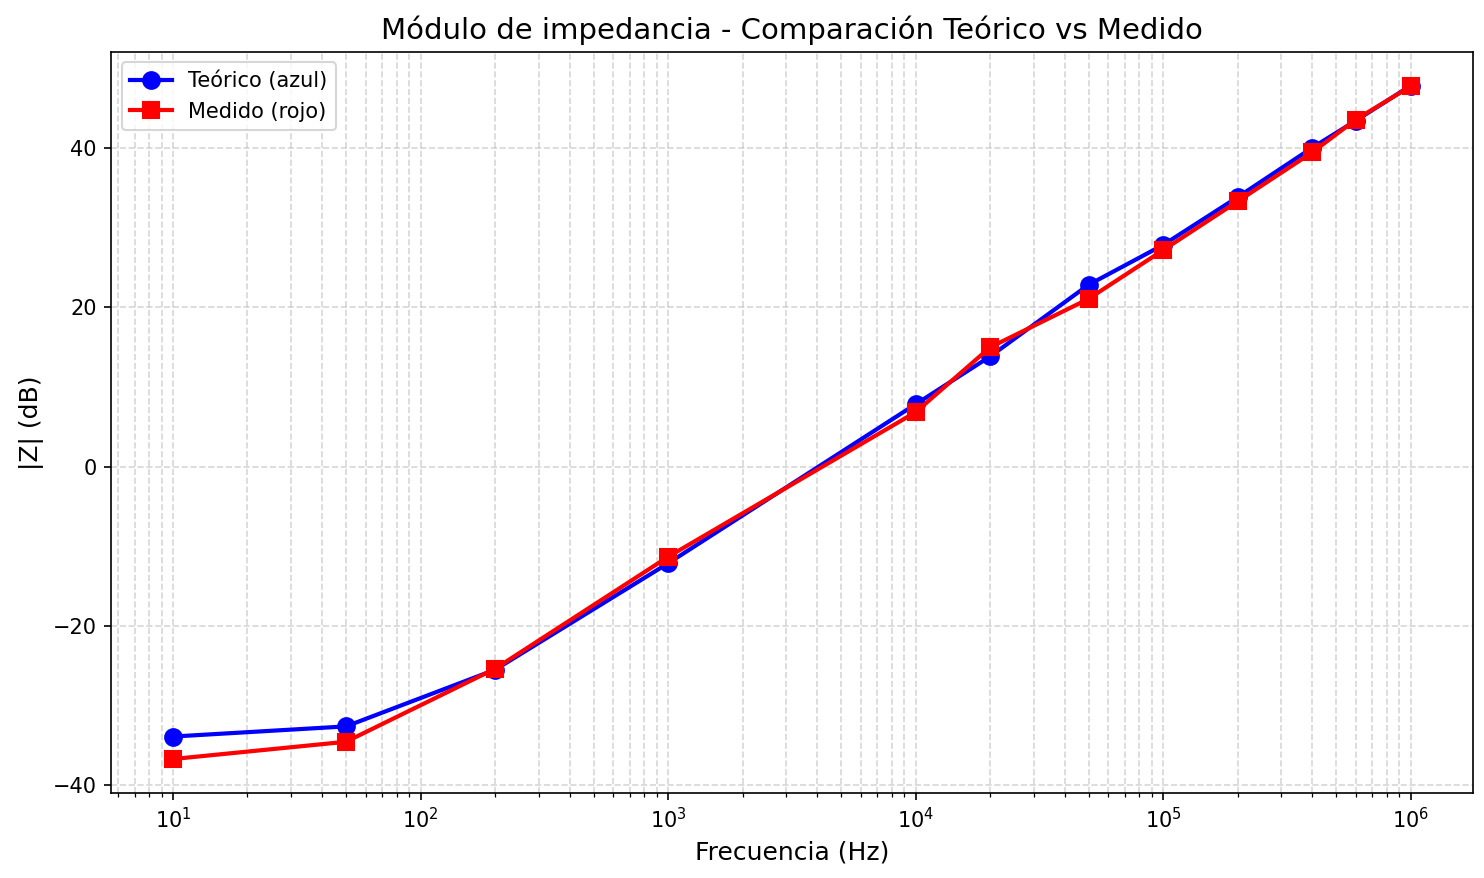
\includegraphics[width=0.8\textwidth]{3_moduloZL.png}
    \caption{Módulo de la impedancia $|Z_L|$ en función de la frecuencia.}
    \label{fig:moduloZL}
\end{figure}

\begin{figure}[H]
    \centering
    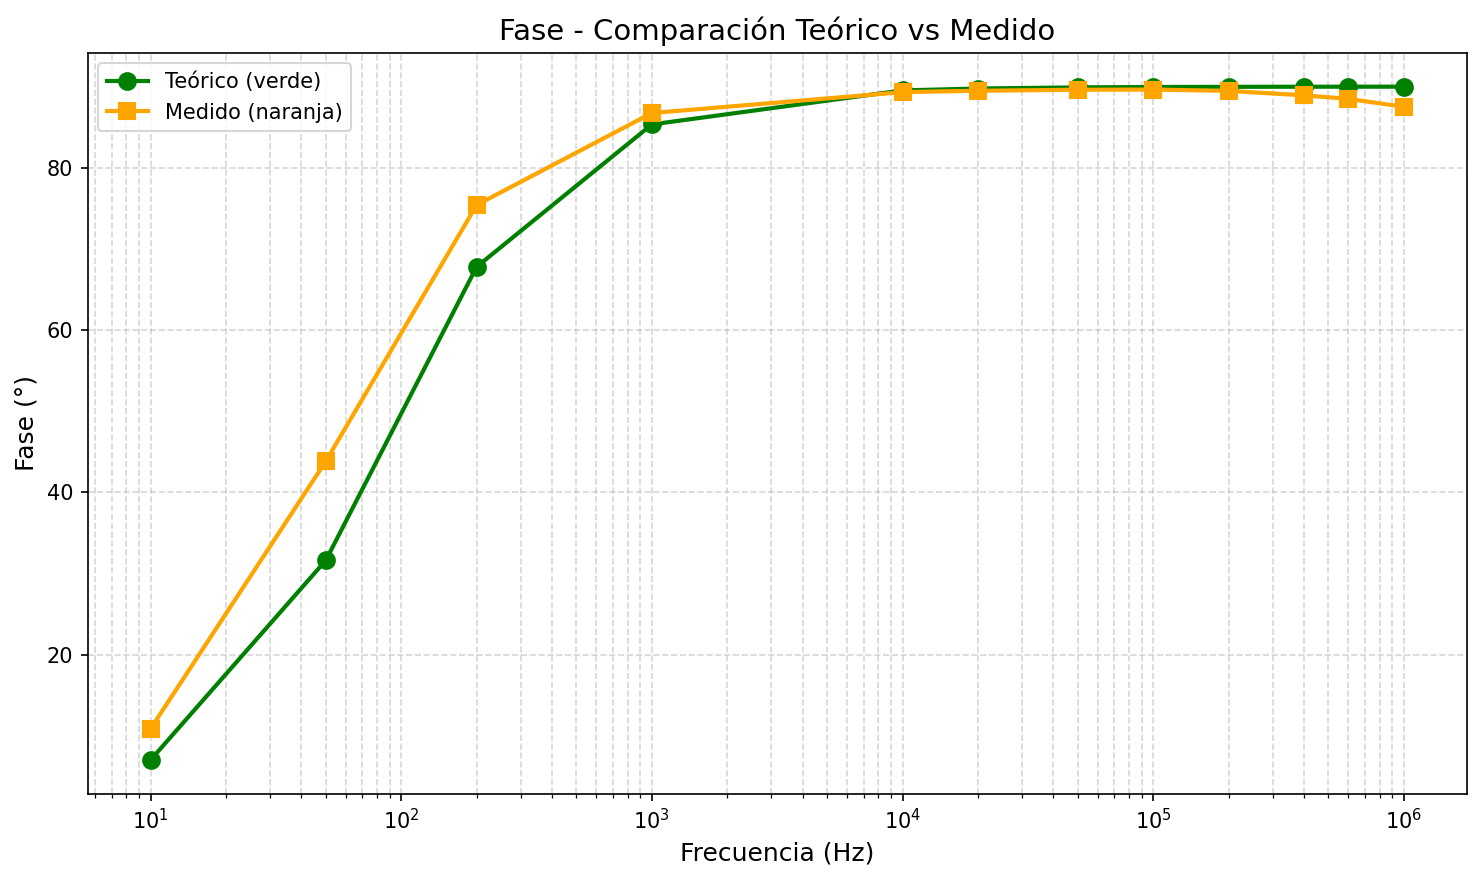
\includegraphics[width=0.8\textwidth]{3_faseZL.png}
    \caption{Fase de la impedancia $|Z_L|$ en función de la frecuencia.}
    \label{fig:faseZL}
\end{figure}

Dada la semejanza entre las curvas teóricas y las medidas, se consideró innecesario complejizar el modelo con la adición de capacitores u otras resistencias. 

Luego, para modelar el capacitor se partió del modelo más simple posible con la resistencia en serie ESR, obtenida mediante
\begin{equation*}
    D=\frac{ESR}{X_C}=\frac{ESR}{\frac{1}{\omega C}} = ESR \cdot 2 \pi f C      \qquad \Rightarrow \qquad       ESR=\frac{D}{2\pi fC}
\end{equation*}


%%%%%%%% EJERCICIO 4 %%%%%%%%%%

\section{Pasabajos}

A partir de la alimentación del circuito con una señal cuadrada de frecuencia 28,2 kHz ($\frac{f_0}{10}$), se obtuvo la siguiente salida en el capacitor dada por la figura~\ref{fig:4_0.png}. 
\begin{figure}[h]
        \centering
        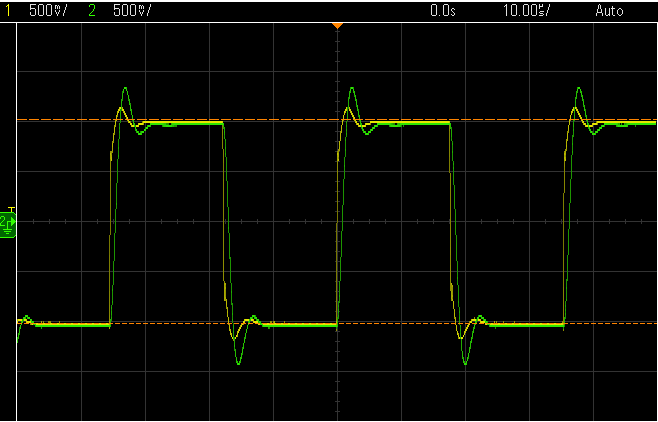
\includegraphics[width=0.5\textwidth]{4_0.png}
        \caption{Verde: Salida de filtro pasabajos ($V_C$) a 28,2 kHz; Amarillo: señal de entrada ($V_{in}$) desde el OpAmp. Escala en tiempo: 10 $\mu s$/div; Escala en tensión: 500 mV/div.}
        \label{fig:4_0.png}
    \end{figure}



% ********* ITEM A *********
\subsection{Respuesta al Escalón}
En base a la medición realizada en la figura \ref{fig:4_0.png}, se obtuvo la siguiente respuesta al escalón: frecuencia de oscilación del transitorio: 238 kHz; tiempo de establecimiento del 5$\%$: $\approx 3,24 \mu$s; sobrepico de 1.38 V. 
Luego, los valores teóricos con los que contrastar los obtenidos experimentalmente son: frecuencia de oscilación del transitorio: 244,5 kHz; tiempo de establecimiento del 5$\%$: $\approx 3,31 \mu$s; sobrepico de 1.31 V. Llegamos a una diferencia de frecuencias de oscilación del transitorio del 2.6\%. La diferencia se puede deber a la tolerancia del capacitor, ya que es el componente de mayor tolerancia (20\%).



% ********* ITEM B *********
\subsection{Salida con Barrido de Frecuencias}
Variando la frecuencia de la señal de entrada, se obtuvieron las siguientes salidas observables en la figura~\ref{fig:comparativa_frecuencias}.
\begin{figure}[h]
    \centering
    % Primera fila
    \begin{subfigure}[b]{0.48\textwidth}
        \centering
        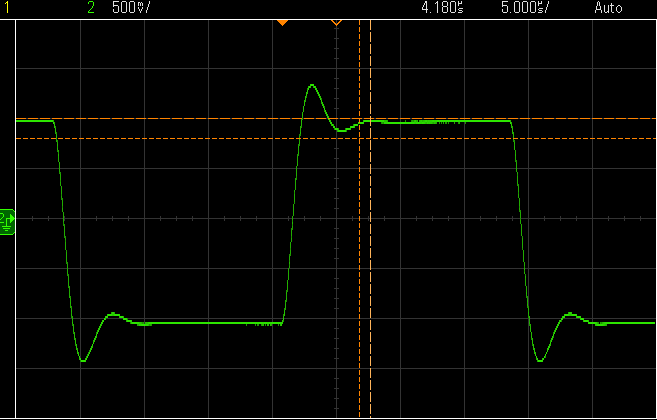
\includegraphics[width=\textwidth]{4b_01.png}
        \caption{Frecuencia: 28,2 kHz}
        \label{fig:f28k}
    \end{subfigure}
    \hfill
    \begin{subfigure}[b]{0.48\textwidth}
        \centering
        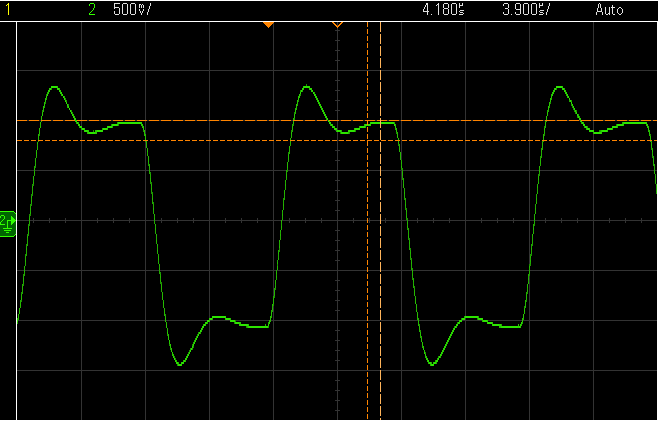
\includegraphics[width=\textwidth]{4b_02.png}
        \caption{Frecuencia: 65 kHz}
        \label{fig:f65k}
    \end{subfigure}

    \vspace{0.5cm} % Espacio entre filas

    % Segunda fila
    \begin{subfigure}[b]{0.48\textwidth}
        \centering
        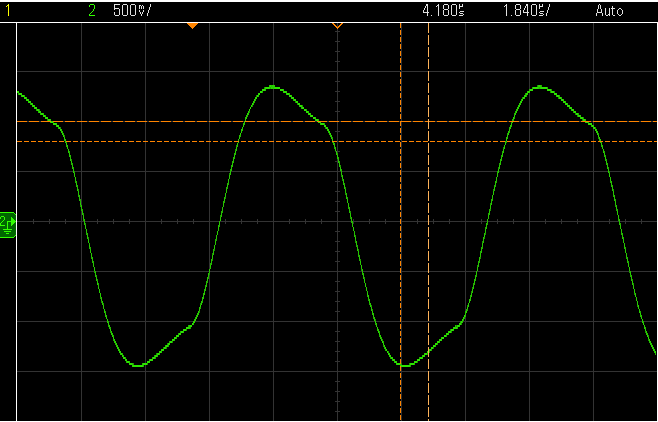
\includegraphics[width=\textwidth]{4b_04.png}
        \caption{Frecuencia: 130 kHz}
        \label{fig:f130k}
    \end{subfigure}
    \hfill
    \begin{subfigure}[b]{0.48\textwidth}
        \centering
        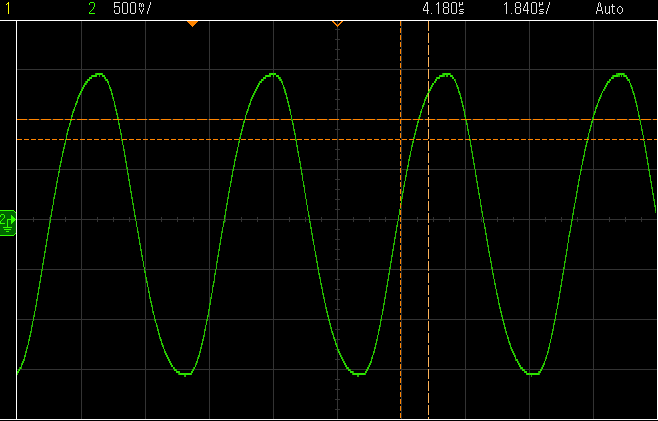
\includegraphics[width=\textwidth]{4b_05.png}
        \caption{Frecuencia: 200 kHz}
        \label{fig:f200k}
    \end{subfigure}

    \caption{Comparación de la respuesta temporal del filtro para distintas frecuencias de entrada. Se observa la atenuación progresiva de la amplitud a medida que aumenta la frecuencia (comportamiento pasabajos). Escala en tiempo: 5$\mu$ s(a), 3,9 $\mu$ s(b), 1,84 $\mu$ s(c) y (d); Escala en tensión: 500 mV/div.}
    \label{fig:comparativa_frecuencias}
\end{figure}
Vemos que a medida que aumenta la frecuencia de la señal de entrada, la amplitud de la salida disminuye, lo cual es consistente con el comportamiento esperado de un filtro pasabajos. Viendo la situación del punto de vista gráfico, se observa que a medida que aumenta la frecuencia, el tiempo de establecimiento disminuye, hasta tener una salida totalmente oscilante. 



% ********* ITEM C *********
\subsection{Cálculo de la Función Transferencia}

A partir del circuito de la figura~\ref{fig:circuito_pasabajos}, la función 
transferencia se obtiene mediante un divisor de impedancias, tomando como 
salida la tensión en el capacitor:

\begin{equation}
    H(s) = \frac{V_o(s)}{V_i(s)} = \frac{Z_C}{Z_L + Z_R + Z_C} 
         = \frac{\dfrac{1}{sC}}{sL + R + \dfrac{1}{sC}}
    \label{eq:H_divisor}
\end{equation}

Multiplicando numerador y denominador por $sC$:

\begin{equation}
    H(s) = \frac{1}{s^2LC + sRC + 1}
    \label{eq:H_s}
\end{equation}

Reescribiendo en forma canónica de segundo orden, con frecuencia natural 
$\omega_0 = \frac{1}{\sqrt{LC}}$ y coeficiente de amortiguamiento 
$\xi = \frac{R}{2}\sqrt{\frac{C}{L}}$:

\begin{equation}
    H(s) = \frac{\omega_0^2}{s^2 + 2\xi\omega_0\, s + \omega_0^2}
    \label{eq:H_canonica}
\end{equation}

Con los valores de los componentes: ($L = \SI{38.3}{\micro\henry}$, 
$C = \SI{8.58}{\nano\farad}$, $R = \SI{68}{\ohm}$), los parámetros resultan:

\begin{equation}
    f_0 = \frac{1}{2\pi\sqrt{LC}} 
        = \frac{1}{2\pi\sqrt{38{,}3\times10^{-6}\cdot 8{,}58\times10^{-9}}} 
        \approx \SI{277.8}{\kilo\hertz}
    \label{eq:f0_pasabajos}
\end{equation}

\begin{equation}
    \xi = \frac{R}{2}\sqrt{\frac{C}{L}} 
        = \frac{68}{2}\sqrt{\frac{8{,}58\times10^{-9}}{38{,}3\times10^{-6}}} 
        \approx 0{,}508
    \label{eq:xi_pasabajos}
\end{equation}

Dado que $\xi < \frac{1}{\sqrt{2}}$, el sistema es subamortiguado y presenta 
sobrepico tanto en la respuesta al escalón como en la respuesta en frecuencia.



% ********* ITEM D *********
\subsection{Diagrama de Bode Teórico-Práctico}
\begin{figure}[H]
        \centering
        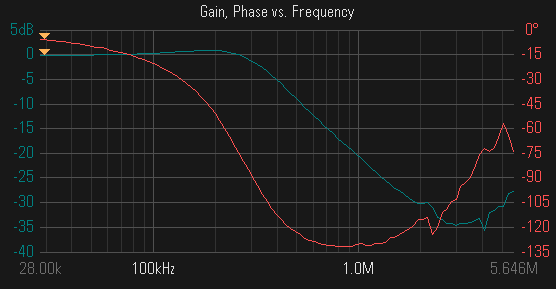
\includegraphics[width=0.7\textwidth]{4d_opam.png}
        \caption{Verde: Salida de filtro pasabajos ($V_C$) a 28,2 kHz; Amarillo: señal de entrada ($V_{in}$) desde el OpAmp. Escala en tiempo: 10 $\mu s$/div; Escala en tensión: 500 mV/div.}
        \label{fig:4d_opam.png}
    \end{figure}


\subsubsection{R = 0 \texorpdfstring{$\Omega$}{pi} }



%%%%%%%%%%%%%%%%%%%%%%%%%%%%%%%%%%%%%%%%%%%
%%%%%%%%%%%%%%%%%%%%%%%%%%%%%%%%%%%%%%%%%%%
%%%%%%%%%%%%%%%%%%%%%%%%%%%%%%%%%%%%%%%%%%%
%   ESTO NO SE SI HACE FALTA              %
%%%%%%%%%%%%%%%%%%%%%%%%%%%%%%%%%%%%%%%%%%%
%%%%%%%%%%%%%%%%%%%%%%%%%%%%%%%%%%%%%%%%%%%
%%%%%%%%%%%%%%%%%%%%%%%%%%%%%%%%%%%%%%%%%%%
\subsection{Respuesta a la Señal Cuadrada}

se uso una señal cuadrada de $f = f_0/10 \approx \SI{27.8}{\kilo\hertz}$ y amplitud 
de $v_{o,\,\text{max}} = \SI{2}{V_{pp}}$. como el periodo de la entrada ($T = \SI{36}{\micro\second}$) es 
diez veces el de oscilacion propia ($T_0 = \SI{3.6}{\micro\second}$), el transitorio llega a terminar en 
cada semiciclo antes de que venga el proximo flanco. por esto, en la salida $v_o(t)$ se ve bien la respuesta
 al escalon y el comportamiento subamortiguado en cada transicion.


Ante un escalón de amplitud $A$, la respuesta temporal de un sistema de segundo 
orden subamortiguado es:

\begin{equation}
    v_o(t) = A\left[1 - \frac{e^{-\xi\omega_0 t}}{\sqrt{1-\xi^2}}
             \sin\!\left(\omega_d t + \phi\right)\right], 
             \quad \phi = \arccos(\xi)
    \label{eq:respuesta_escalon}
\end{equation}

donde la frecuencia de oscilación del transitorio es:

\begin{equation}
    \omega_d = \omega_0\sqrt{1-\xi^2} \implies 
    f_d = f_0\sqrt{1-\xi^2} 
        = \SI{277.8}{\kilo\hertz}\cdot\sqrt{1-0{,}508^2} 
        \approx \SI{240.8}{\kilo\hertz}
    \label{eq:fd}
\end{equation}

El sobrepico máximo, que ocurre en $t_p = \pi/\omega_d$, vale:

\begin{equation}
    M_P = e^{-\pi\xi/\sqrt{1-\xi^2}} 
        = e^{-\pi \cdot 0{,}508/\sqrt{1-0{,}508^2}} 
        \approx 0{,}163
    \label{eq:MP}
\end{equation}

Es decir, la salida supera el valor final en un $16{,}3\%$ del escalón aplicado.


%%%%%%%% EJERCICIO 5 %%%%%%%%%%

\section{Pasaaltos, Pasabandas y Rechazabandas}

Es importante mencionar antes de iniciar el análisis que puesto a que los tres filtros tienen los mismo componentes y viendo las ecuaciones deducidas en el anexo (de las cuales se hablará más adelante), todos los circuitos poseen la misma frecuencia de corte. 
\begin{figure}[h!]
    \centering

    \begin{minipage}[b]{0.32\textwidth}
        \centering
        \resizebox{\linewidth}{!}{
        \begin{tikzpicture}[transform shape]
	\draw (-11, 4) to[american voltage source] (-11, 2);
	\node[buffer, xscale=0.66, yscale=0.66] at (-10.038, 4){};
	\draw (-11, 4) -- (-10.5, 4);
	\draw (-9.576, 4) to[american resistor, l={$R$}] (-7.988, 4);
	\draw (-7.988, 4) to[capacitor, l={$C$}] (-6.5, 4);
	\draw (-6.5, 4) to[american inductor, l={$L$}] (-6.5, 2);
	\draw (-11, 2) -- (-6.5, 2);
	\node at (-6.375, 4.125){$v_{out}$};
	\node at (-11, 4.125){$v_{in}$};
        \end{tikzpicture}}
        \caption{Pasaaltos}
        \label{fig:pasaaltos}
    \end{minipage}
    \hfill
    \begin{minipage}[b]{0.32\textwidth}
        \centering
        \resizebox{\linewidth}{!}{
        \begin{tikzpicture}[transform shape]
	\draw (-11, 4) to[american voltage source] (-11, 2);
	\node[buffer, xscale=0.66, yscale=0.66] at (-10.038, 4){};
	\draw (-11, 4) -- (-10.5, 4);
	\draw (-6.5, 4) to[american resistor, l={$R$}] (-6.5, 2);
	\draw (-7.988, 4) to[capacitor, l={$C$}] (-6.5, 4);
	\draw (-9.576, 4) to[american inductor, l={$L$}] (-8, 4);
	\draw (-11, 2) -- (-6.5, 2);
	\node at (-6.375, 4.125){$v_{out}$};
	\node at (-11, 4.125){$v_{in}$};
        \end{tikzpicture}}
        \caption{Pasabandas}
        \label{fig:pasabandas}
    \end{minipage}
    \hfill
    \begin{minipage}[b]{0.32\textwidth}
        \centering
        \resizebox{\linewidth}{!}{
        \begin{tikzpicture}[transform shape]
	\draw (-11, 4) to[american voltage source] (-11, 2);
	\node[buffer, xscale=0.66, yscale=0.66] at (-10.038, 4){};
	\draw (-11, 4) -- (-10.5, 4);
	\draw (-9.576, 4) to[american resistor, l={$R$}] (-6.5, 4);
	\draw (-6.5, 2.75) to[capacitor, l={$C$}] (-6.5, 2);
	\draw (-6.5, 4) to[american inductor, l={$L$}] (-6.5, 2.75);
	\draw (-11, 2) -- (-6.5, 2);
	\node at (-6.375, 4.125){$v_{out}$};
	\node at (-11, 4.125){$v_{in}$};
        \end{tikzpicture}}
        \caption{Notch}
        \label{fig:notch}
    \end{minipage}

\end{figure}
Primero analizaremos la respuesta de cada filtro en función del tiempo. 

\begin{figure}[H]
    \centering

    \begin{minipage}[b]{0.32\textwidth}
        \centering
        \includegraphics[page=2, width=\linewidth]{Graficos.pdf}
        \caption{Pasaaltos}
        \label{fig:pasaaltostiempo}
    \end{minipage}
    \hfill
    \begin{minipage}[b]{0.32\textwidth}
        \centering
        \includegraphics[page=3, width=\linewidth]{Graficos.pdf}
        \caption{Pasabandas}
        \label{fig:pasabandastiempo}
    \end{minipage}
    \hfill
    \begin{minipage}[b]{0.32\textwidth}
        \centering
        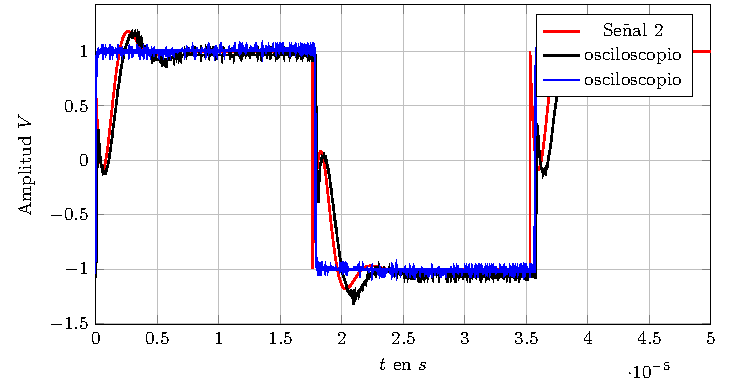
\includegraphics[page=1, width=\linewidth]{Graficos.pdf}
        \caption{Notch}
        \label{fig:notchtiempo}
    \end{minipage}

\end{figure}
Al observar la gráfica de todas las señales, se puede observar que hay una gran correlación en la gráfica obtenida mediante el osciloscopio y la simulada en el ltspice. Una de las principales diferencias que se pueden observar en las tres señales es el desfase en el tiempo. La explicación de esto se debe a la existencia de un buffer a la entrada del circuito el cual añade un efecto de slew-rate. Esto es que el buffer limita la maxima pendiente de subida que la señal puede tener, limitando la velocidad de carga del circuito. Esto termina desenbocando en un desfase en el tiempo del circuito que se puede observar en las tres graficas \ref{fig:pasaaltostiempo}, \ref{fig:pasabandastiempo} y \ref{fig:notchtiempo}



%%%%%%%% EJERCICIO 6 %%%%%%%%%%

\section{Medición del Factor de Calidad}

\subsection{Cálculo Analítico}

El factor de calidad $Q$ para un circuito RLC serie se define como:

\begin{equation}
    Q = \frac{1}{R}\sqrt{\frac{L}{C}} = \frac{\omega_0 L}{R}
    \label{eq:Q_def}
\end{equation}

Utilizando los valores nominales de los componentes 
($L = \SI{38.76}{\micro\henry}$, $C = \SI{8.2}{\nano\farad}$, $R = \SI{68}{\ohm}$):

\begin{equation}
    Q_{\text{nominal}} = \frac{1}{68}\sqrt{\frac{38{,}76 \times 10^{-6}}{8{,}2 \times 10^{-9}}} = 1{,}00
    \label{eq:Q_nominal}
\end{equation}

Utilizando los valores medidos experimentalmente 
($L = \SI{38.3}{\micro\henry}$ a $f = \SI{200}{\kilo\hertz}$, $C = \SI{8.58}{\nano\farad}$):

\begin{equation}
    Q_{\text{teórico}} = \frac{1}{68}\sqrt{\frac{38{,}3 \times 10^{-6}}{8{,}58 \times 10^{-9}}} = 1{,}022
    \label{eq:Q_teo}
\end{equation}

\subsection{Métodos Empíricos y Selección del de Menor Error}

Se analizaron dos métodos para medir $Q$ experimentalmente con el osciloscopio 
y el generador de señales.

\subsubsection*{Método A — Frecuencia del pico de amplitud}

En la configuración pasabajos (salida en el capacitor), la ganancia presenta un 
máximo no en $f_0$ sino en una frecuencia ligeramente inferior, dada por:

\begin{equation}
    f_{\text{pico}} = f_0 \sqrt{1 - \frac{1}{2Q^2}}
    \label{eq:f_pico}
\end{equation}

Midiendo experimentalmente $f_{\text{pico}}$ y conociendo $f_0$, se puede 
despejar $Q$ de la ecuación~\ref{eq:f_pico}. La ventaja de este método es que 
$f_{\text{pico}}$ es localizable ajustando la frecuencia del generador hasta 
maximizar la amplitud de $V_{out}$. Sin embargo, cualquier imprecisión en la 
determinación de $f_0$ se propaga directamente al cálculo de $Q$, siendo este 
su principal fuente de error.

\subsubsection*{Método B — Razón de amplitudes en resonancia}

En la frecuencia de resonancia $f_0$, la función de transferencia del capacitor 
tiene módulo igual a $Q$:

\begin{equation}
    \left|H(j\omega_0)\right| = Q \implies Q = \frac{\left|V_{out}(f_0)\right|}{\left|V_{in}(f_0)\right|}
    \label{eq:Q_metodo_B}
\end{equation}

Este método requiere únicamente medir las amplitudes de $V_{in}$ y $V_{out}$ 
simultáneamente en $f_0$ con los dos canales del osciloscopio. Al tratarse de 
un cociente de amplitudes en un único punto de frecuencia, el error queda 
limitado a la resolución vertical del instrumento, sin depender de un barrido 
fino de frecuencias. Por lo anterior, el Método B es el que introduce 
menor error y fue adoptado como método principal.

Para localizar $f_0$ con mayor precisión previo a aplicar el Método B, se 
utilizó la condición de fase: en $\omega_0$ la tensión en el capacitor se 
encuentra desfasada exactamente $-90°$ respecto de $V_{in}$. Alimentando el 
circuito con una señal sinusoidal de \SI{1}{V_{pp}}, se varió la frecuencia 
hasta observar en el osciloscopio que ambas sinusoides presentaban un desfasaje 
de aproximadamente $90°$, como se muestra en la figura~\ref{fig:desfasaje_f0}.

\subsection{Resultados Experimentales}

\subsubsection*{Determinación de \texorpdfstring{$f_0$}{f0}}

Mediante el procedimiento de desfasaje descripto se obtuvo:

\begin{equation}
    f_{0,\,\text{medido}} = \SI{273}{\kilo\hertz} \qquad 
    f_{0,\,\text{teórico}} = \frac{1}{2\pi\sqrt{LC}} = \SI{282.7}{\kilo\hertz}
    \label{eq:f0_comparacion}
\end{equation}

La diferencia del $3{,}4\%$ es consistente con las tolerancias de los 
componentes, en particular el capacitor de poliéster con tolerancia del $20\%$.

\begin{figure}[H]
    \centering
    %\includegraphics[width=0.7\textwidth]{imagenes/desfasaje_f0.png}
    \caption{Desfasaje de $\approx 90°$ entre $V_{in}$ (amarillo) y $V_{out}$ 
             (verde) a $f_0 = \SI{273}{\kilo\hertz}$, confirmando la 
             frecuencia de resonancia.}
    \label{fig:desfasaje_f0}
\end{figure}

\subsubsection*{Método A}

Buscando el máximo de amplitud de $V_{out}$ mediante barrido de frecuencia, 
se halló la frecuencia del pico:

\begin{equation}
    f_{\text{pico}} \approx \SI{197}{\kilo\hertz}
    \label{eq:f_pico_medido}
\end{equation}

Despejando $Q$ de la ecuación~\ref{eq:f_pico} con los valores de las 
ecuaciones~\ref{eq:f0_comparacion} y~\ref{eq:f_pico_medido}:

\begin{equation}
    Q_A = \frac{1}{\sqrt{2\left[1-\left(\dfrac{f_{\text{pico}}}{f_0}\right)^2\right]}} 
        = \frac{1}{\sqrt{2\left[1-\left(\dfrac{197}{273}\right)^2\right]}} 
        = 0{,}995
    \label{eq:QA}
\end{equation}

\begin{figure}[H]
    \centering
    %\includegraphics[width=0.7\textwidth]{imagenes/metodo_A_pico.png}
    \caption{Medición de $f_{\text{pico}} \approx \SI{197}{\kilo\hertz}$ 
             en el osciloscopio. Se observa la amplitud máxima de $V_{out}$ 
             (canal 1, verde) respecto de $V_{in}$ (canal 2, amarillo).}
    \label{fig:metodo_A}
\end{figure}

\subsubsection*{Método B}

Se midieron las amplitudes pico a pico de $V_{out}$ y $V_{in}$ en $f_0$ 
con los cursores del osciloscopio, tal como se ilustra en la 
figura~\ref{fig:metodo_B}. Aplicando la ecuación~\ref{eq:Q_metodo_B}:

\begin{equation}
    Q_B = \frac{\left|V_{out}(f_0)\right|}{\left|V_{in}(f_0)\right|} = 1{,}05
    \label{eq:QB}
\end{equation}

\begin{figure}[H]
    \centering
    %\includegraphics[width=0.7\textwidth]{imagenes/metodo_B_amplitudes.png}
    \caption{Medición de amplitudes en $f_0 = \SI{273}{\kilo\hertz}$ 
             mediante cursores. Canal 1 (verde): $V_{out}$; 
             Canal 2 (amarillo): $V_{in}$.
             El cociente de amplitudes da $Q_B = 1{,}05$.}
    \label{fig:metodo_B}
\end{figure}

\subsection{Comparación y Análisis}

En la tabla~\ref{tab:Q_comparacion} se resumen los valores obtenidos 
por cada método.

\begin{table}[H]
    \centering
    \caption{Comparación de valores del factor de calidad $Q$.}
    \label{tab:Q_comparacion}
    \begin{tabular}{lc}
        \toprule
        Método & $Q$ \\
        \midrule
        Nominal (valores de catálogo)       & $1{,}00$ \\
        Teórico (componentes medidos)       & $1{,}022$ \\
        Método A (frecuencia del pico)      & $0{,}995$ \\
        Método B (razón de amplitudes)      & $1{,}05$  \\
        \bottomrule
    \end{tabular}
\end{table}

Ambos métodos arrojan resultados dentro del $4\%$ del valor teórico calculado 
con los componentes medidos, lo cual es aceptable ya que el inductor presenta una resistencia 
serie parásita $r_L$ que incrementa el $R$ efectivo del circuito, reduciendo el 
$Q$ real respecto del nominal.


El método B es el más práctico y repetible debido a que introduce menor error. En particular, en este
escenario solo basta con hacer el cociente de las amplitudes en el entorno cercano a la fracuencia natural
del sistema. Por otra parte, el método A induce mayor error debido a que es más sensible respecto a la 
variable del $f?0$. Esto se denota en la expresión~\ref{eq:f_pico}, la cual involucra una diferencia de
cuadrados de frecuencias relativamente cercanas.




%%%%%%%%%%% ANEXO %%%%%%%%%%%

\section{Anexo}

\subsection{Deducciones matemáticas}
\label{subsec:Deduccionesmat}
En la deducción de los filtros, se ignora el opamp. Esto se realiza ya que la idea del opamp es aislar el circuito de la resistencia interna del generador para tratar de conseguir el circuito que se deduce aproximación. \\
\subsubsection{Filtro pasabandas}
\label{subsec:eqpasabandas}
Partiendo de la figura \ref{fig:pasabandas}, se planteo un divisor resistivo:

\begin{align*}
   H(s) &= \frac{R}{SL+\frac{1}{SC}+R}\\
   H(s) &= \frac{sRC}{s^2LC+ sCR +1}
\end{align*}

De aquí se deduce que su frecuencia de corte es $f_0 = \frac{1}{2\pi \sqrt{LC}}$

\subsubsection{Filtro pasaaltos}
\label{subsec:eqpasaaltos}
Partiendo de la figura \ref{fig:pasaaltos}, se planteo un divisor resistivo:
\begin{align*}
   H(s) &= \frac{sL}{SL+\frac{1}{SC}+R}\\
   H(s) &= \frac{s^2LC}{s^2LC+ sCR +1}
\end{align*}

De aquí se deduce que su frecuencia de corte es $f_0 = \frac{1}{2\pi \sqrt{LC}}$

\subsubsection{Filtro notch}
\label{subsec:eqpasabandas}
Partiendo de la figura \ref{fig:notch}, se planteo un divisor resistivo:
\begin{align*}
   H(s) &= \frac{sL+\frac{1}{sC}}{SL+\frac{1}{SC}+R}\\
   H(s) &= \frac{s^2LC+1}{s^2LC+ sCR +1}
\end{align*}

De aquí se deduce que su frecuencia de corte es $f_0 = \frac{1}{2\pi \sqrt{LC}}$

\subsection{Polo de medicion}
\label{subsec:eqpolo}
Al observar la figura \ref{fig:pasabandas}, si uno conecta una punta de osciloscopio sobre la salida, estas introducen una capacitancia parasita que introduce un polo. Esto se puede demostrar analíticamente de la siguiente forma:

\begin{align*}
H(s) &= \frac{R//C_2}{sL + \frac{1}{sC_1} + R//C_2}\\
H(s) &= \frac{\frac{R}{1+sRC_2}}{sL + \frac{1}{sC_1} + \frac{R}{1+sRC_2}}
\end{align*}

Con $C_1$ la capacidad del capacitor del circuito y $C_2$ la capacitancia del capacitor de las puntas del osciloscopio.\par




        
\end{document}
